% \documentclass{article}
% %\usepackage[english]{babel}%
% \usepackage{graphicx}
% \usepackage{tabulary}
% \usepackage{tabularx}
% \usepackage[normalem]{ulem}
% \usepackage{cancel}
% \usepackage{tikz} 
% \usepackage{pdflscape}
% \usepackage{colortbl}
% \usepackage{lastpage}
% \usepackage{multirow}
% \usepackage{enumerate}
% \usepackage[shortlabels]{enumitem}
% \usepackage{color,soul}
% \usepackage{pdflscape}
% \usepackage{hyperref}
% %\usepackage[table]{xcolor}
% \usepackage{rotating}
% \usepackage{amsmath}
% \usepackage{fixltx2e}
% \usepackage{framed}
% \usepackage{mdframed}
% \usepackage[T1]{fontenc}
% \usepackage[utf8]{inputenc}
% \usepackage{textcomp}
% \usepackage{siunitx}
% \usepackage{ifthen}
% \usepackage{fancyhdr}
% \usepackage{gensymb}
% \usepackage{newunicodechar}
% \usepackage[document]{ragged2e}
% \usepackage[margin=1in,top=1.1in,headheight=57pt,headsep=0.1in]
% {geometry}
% \usepackage{ifthen}
% \usepackage{fancyhdr}
% \everymath{\displaystyle}
% \usepackage[document]{ragged2e}
% \usepackage{fancyhdr}
% \everymath{\displaystyle}
% \usepackage{empheq}

% \usepackage[most]{tcolorbox}

% \usepackage{booktabs} % Required for nicer horizontal rules in tables


% \usepackage{enumitem}

% %\usepackage[table,xcdraw]{xcolor}
% \usetikzlibrary{arrows}
% \linespread{2}%controls the spacing between lines. Bigger fractions means crowded lines%
% %\pagestyle{fancy}
% %\usepackage[margin=1 in, top=1in, includefoot]{geometry}
% %\everymath{\displaystyle}
% \linespread{1.3}%controls the spacing between lines. Bigger fractions means crowded lines%
% %\pagestyle{fancy}
% \pagestyle{fancy}
% \setlength{\headheight}{56.2pt}

% \definecolor{myblue}{rgb}{.8, .8, 1}
% \newcommand*\mybluebox[1]{%
% \colorbox{myblue}{\hspace{1em}#1\hspace{1em}}}

% \chead{\ifthenelse{\value{page}=1}{
\includegraphics[scale=0.3]{SCC}\\ \textbf \textbf Wastewater Constituents Analysis \& Laboratory Methods}}
% \rhead{\ifthenelse{\value{page}=1}{}{}}
% \lhead{\ifthenelse{\value{page}=1}{}{Wastewater Constituents Analysis \& Laboratory Methods}}
% \rfoot{\ifthenelse{\value{page}=1}{Module 1: WATR 048 - Spring 2019}{Module 1: WATR 048 - Spring 2019}}

% \lfoot{Shabbir Basrai}
% \cfoot{Page \thepage\ of \pageref{LastPage}}
% \renewcommand{\headrulewidth}{2pt}
% \renewcommand{\footrulewidth}{1pt}
% \begin{document}
% %\begin{empheq}[box=\mybluebox]{align}
% %a&=b\\
% %E&=mc^2 + \int_a^a x\, dx
% %\end{empheq}

% \newlist{steps}{enumerate}{1} % Defines "Steps" for enumerate as Step 1, Step 2 etc.
% \setlist[steps, 1]{label = Step \arabic*:} % Defines "Steps" for enumerate as Step 1, Step 2 etc.

% \setlist{nolistsep} % Reduce spacing between bullet points and numbered lists


%_______________________________________________________________________________________________________________________________________%
%----------------------------------------------------------------------------------------------%
\chapterimage{Week3Clarifier1.jpg} % Chapter heading image

\chapter{Primary Treatment}

%\section{Background}\index{Background}
\begin{itemize}
\item Synonyms:  primary treatment basin, primary clarifier, sedimentation basin, primaries, clarifier

	
		\item Primary treatment is after preliminary treatment and 				before secondary treatment
		\item Its two main objectives are: 
			\begin{itemize}
				\item Remove settleable solids
				\item Remove floatable solids
			\end{itemize}
		\item This is a physical process which relies on the physical 			properties - how heavy or light the suspended solids particles 		are to effect its separation
		\item Provides quiescent conditions for the influent 					wastewater for the heavier solids to settle and the lighter 			solids to float
		\item Removes settleable solids and floatables
		\item Settled solids are removed as sludge from the bottom of 			the clarifier
		\item Floatable solids including oil and grease are also 				removed, as scum from the surface\\
		\item The shape of the primary clarifier is either rectangular 		or circular
	
		\item Effective solids removal in the primary clarifiers will 			reduce the loading on the expensive secondary treatment 				process.
		\item The amount of solids removed during primary treatment 			may be enhanced by chemical addition - ferric or ferrous 				chloride as a coagulant and anionic polymer as the flocculant.  		This is called Chemically Enhanced Primary Treatment (CEPT).
\item \textbf{Typical Removal Rates:}\\
\begin{itemize}
\item \hspace{10mm} BOD removal – 25\% to 40\% and about 60\% with CEPT
\item \hspace{10mm} Suspended solids (SS) removal – 40\% to 60\% and about 75\% with CEPT
\item \hspace{10mm} Settleable Solids removal - $>$90\%
\end{itemize}
\end{itemize}
\clearpage
			\begin{center}
				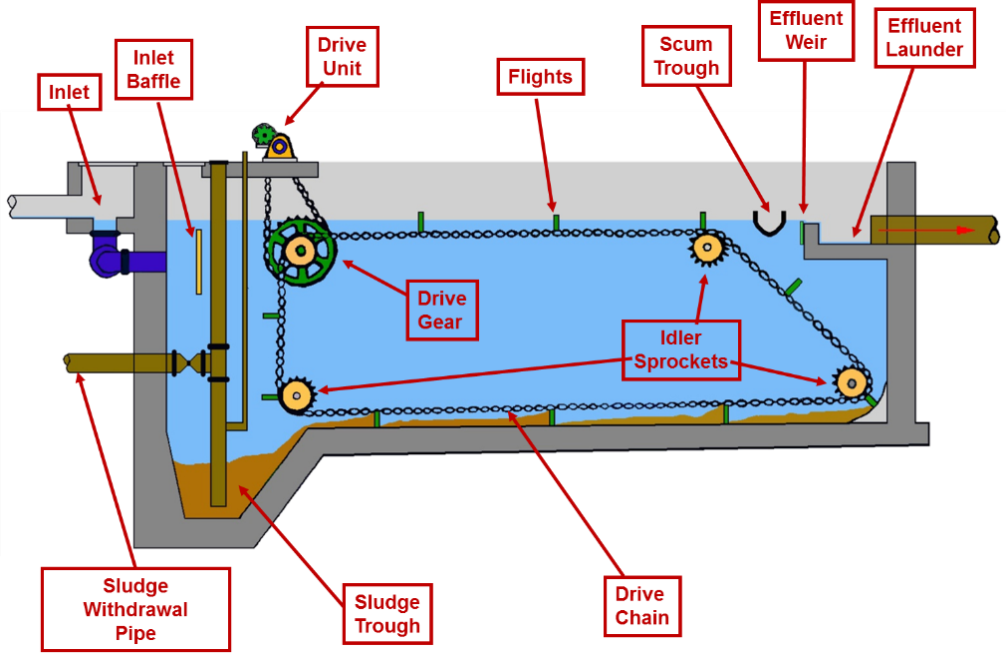
\includegraphics[scale=0.9]{RectangularClarifier}\\
				Cross section of a Rectangular Clarifier\\

				
\includegraphics[scale=0.1]{Blank}\\
				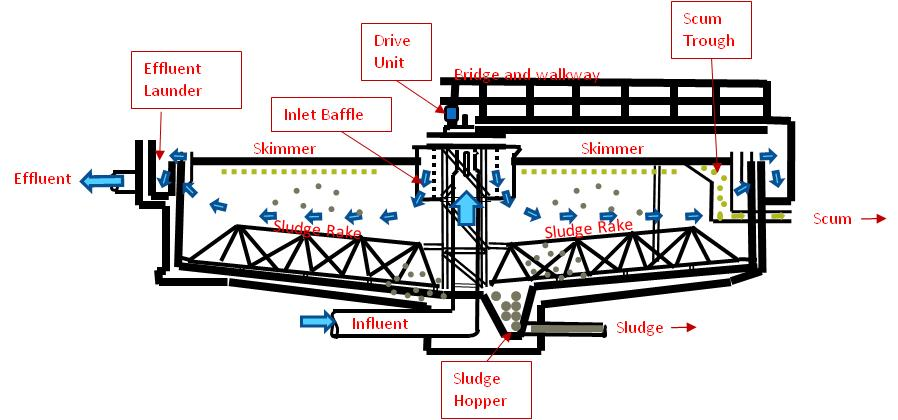
\includegraphics[scale=0.6]{CircularClarifierAI}\\
				Schematic cross section of a circular clarifier\\
				
\includegraphics[scale=0.1]{Blank}\\
				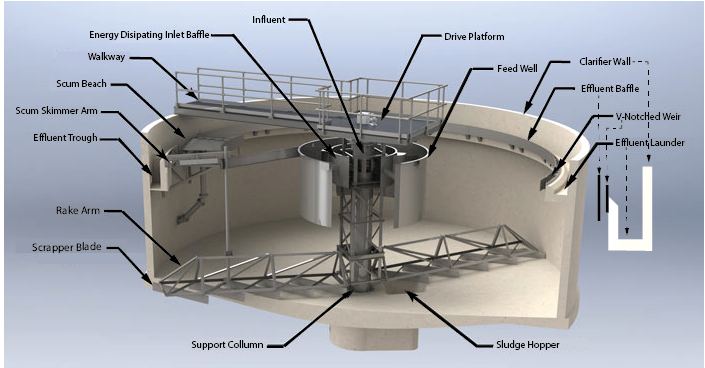
\includegraphics[scale=0.5]{CircularClarifier3}\\
				Cross section of a circular clarifier\\
			\end{center}
				
\includegraphics[scale=0.03]{Blank}\\


\section{Clarifier Zones}\index{Clarifier Zones}
				
\subsection{Inlet Zone}\index{Inlet Zone}		
				\begin{itemize}
					\item Inlet Zone is where the water enters the end 					of a rectangular tank, or the center of a circular 					or square tank.
					\item The Inlet Zone is designed to accomplish two 					objectives:
						\begin{enumerate}
							\item Reduce the velocity (dissipate 									energy in the incoming water)
							\item Distribute the flow evenly
						\end{enumerate}
					\item The inlet zone is equipped with a baffle.  					Inlet baffle reduces the velocity of the 							influent flow, prevent short circuiting which 							could cause solids being carried over to secondary 					treatment.  
						\begin{itemize}
							\item Circular tanks are equipped with a 								collar-type circular baffle that directs 								the water down as it enters the center of 								the tank.
							\item Rectangular tanks will have a plate 								baffle in front of the opening for the 									wastewater flow into the clarifier and 									another baffle just upstream - a 										perforated wall or a picket fence type 									baffle that spreads the water laterally 								across the inlet end of the tank.\\

\begin{figure}[h!]
  \centering
  \begin{subfigure}[b]{0.4\linewidth}
    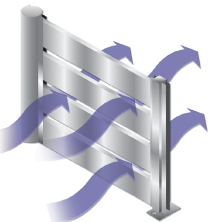
\includegraphics[width=0.8\linewidth]{InfluentBaffle}
    \caption{Rectangular clarifier influent baffle}
  \end{subfigure}
  \hspace{1cm}
  \begin{subfigure}[b]{0.4\linewidth}
    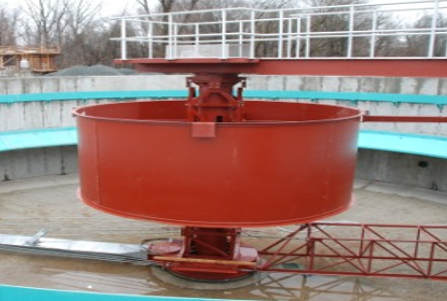
\includegraphics[width=\linewidth]{CircularClarifierInfluentBaffle}
    \caption{Circular clarifier influent baffle}
  \end{subfigure}
\end{figure}	
	
%							\begin{center}
%							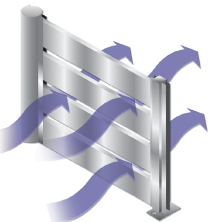
\includegraphics[scale=0.65]												{InfluentBaffle}\\
%							Rectangular clarifier influent baffle
%							\end{center}
%							
%														\begin{center}
%							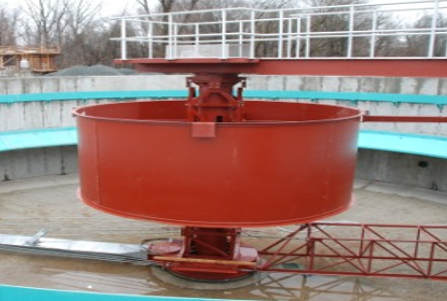
\includegraphics[scale=0.65]												{CircularClarifierInfluentBaffle}\\
%							Circular clarifier influent baffle
%							\end{center}	
						\end{itemize}
				\end{itemize}

\subsection{Settling Zone}\index{Settling Zone}
			\begin{itemize}
				\item This is the largest portion of the tank where 					solids settle.
				\item The water velocity is reduced to 0.03-0.05 fps 					and the detention time is about 1.5 to 2 hours. 
				\item A clarifier is said to be short circuiting if 					the velocity of the water is greater in some sections 					than in others. The water passing through the higher 					velocity region will have a reduced detention time and 				settleable solids will carry through with this water 					as it goes over the weir.  Short circuiting is 							prevented by appropriately designing inlet baffles and weir plates (at the Outlet Zone).
			\end{itemize}

\subsection{Sludge Zone}\index{Sludge Zone}
			\begin{itemize} 
				\item Sludge zone is the bottom of the tank where the 					settled sludge collects and compacts.
				\item Sludge blanket depth should be measured and 						sludge should be removed at least every shift. A 						desirable blanket depth is typically established and 					the sludge pumping rate and regimen is established to 					maintain that desired sludge blanket level.
				\item Sludge rakes push the sludge to one end or the 					center of the tank so that it can be pumped out. 
				\item The rake drive is usually equipped with a torque 				indicator. A shear pin in the drive shaft will break 					to prevent damage to the gearbox or drive shaft. 
				\item Failure to remove sludge often enough will 						result in the sludge becoming septic releasing gas 						bubbles which hinders the sludge settling and also 						result in causing odor problems.
				\item The sludge from the primary clarifiers needs to 					be stabilized prior to its disposal.  The sludge 						(solids) from the primary clarifiers are mixed with 					the solids from the secondary treatment process and 					stabilized typically using a sludge digestion process. 
			\end{itemize}
\subsection{Skimming Zone}\index{Skimming Zone}

			\begin{itemize}
				\item The skimming zone is at the surface of the tank 					for scum removal
				\item Lighter solids and greases float to the surface 					of the clarifier as scum
				\item In Circular Clarifiers:  Floating matter is 						skimmed by a skimmer arm that is supported by the 						sludge rake and rotates with it around the tank. The 					floating matter is pushed over the beach plate by the 					wipers attached to the skimmer arm and into a scum box 				attached to the tank wall.\\
				\item In Rectangular Clarifiers:  The flights act as 							skimmers when the chain brings them to the surface and 				pushes the scum towards the scum troughs.  The scum 					trough may be designed to rotate (tip) periodically 					for the scum to flow in from the water surface.\\
							
				\item The scum collected from the primary clarifiers is sent 				to the digester for treatment along with the sludge 					removed.\\ 

				\vspace{1cm}
									\begin{center}
					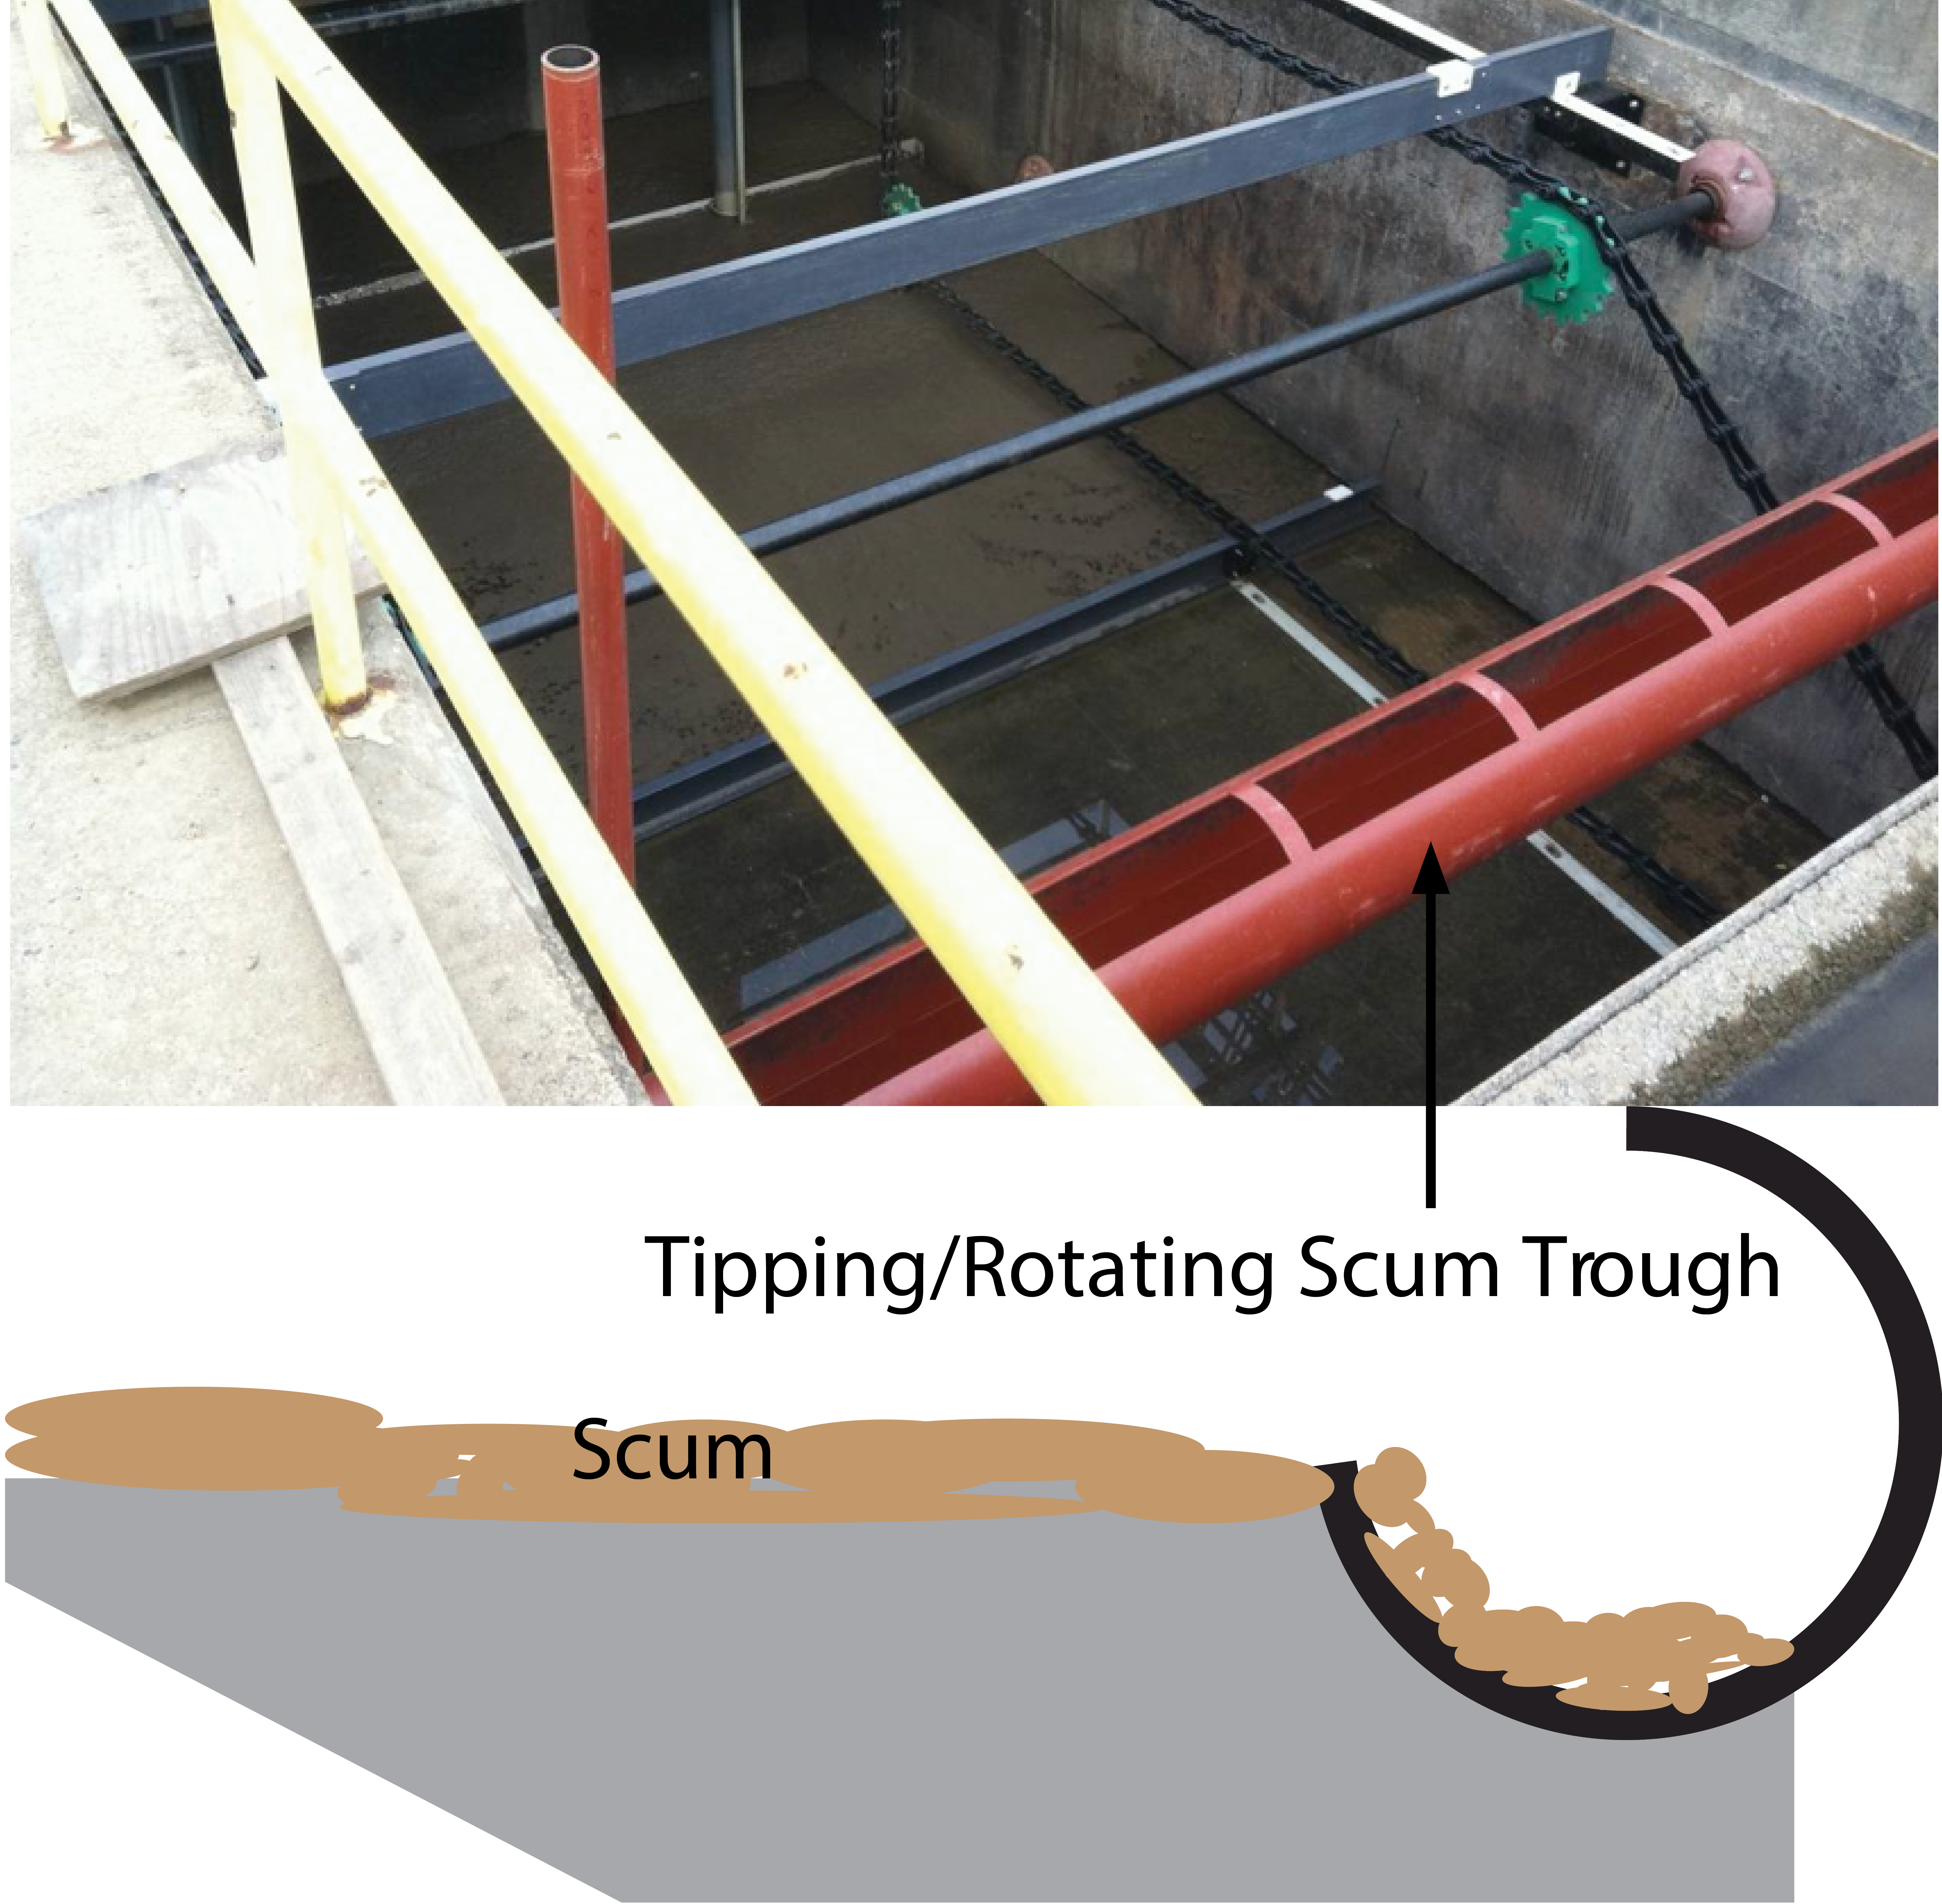
\includegraphics[scale=0.06]{RotatingScumTrough}\\
					Rectangular clarifier scum trough\\
									
\includegraphics[scale=0.02]{Blank}\\
				\end{center}	

				\item The flights in the rectangular clarifier are supported 				at the top by two parallel rails running along the 						length of the clarifier.\\
				\item There are wear plates (strips) installed at the 						clarifer bottom and on top of the rails to prevent the 				flights from riding directly on those surfaces.  To 					reduce friction, the flights have a wearing shoe 						attached.  
				\item Both the wear strip and the wearing shoe 					are disposable items and are replaced at fixed 							intervals.\\			
				\begin{center}
					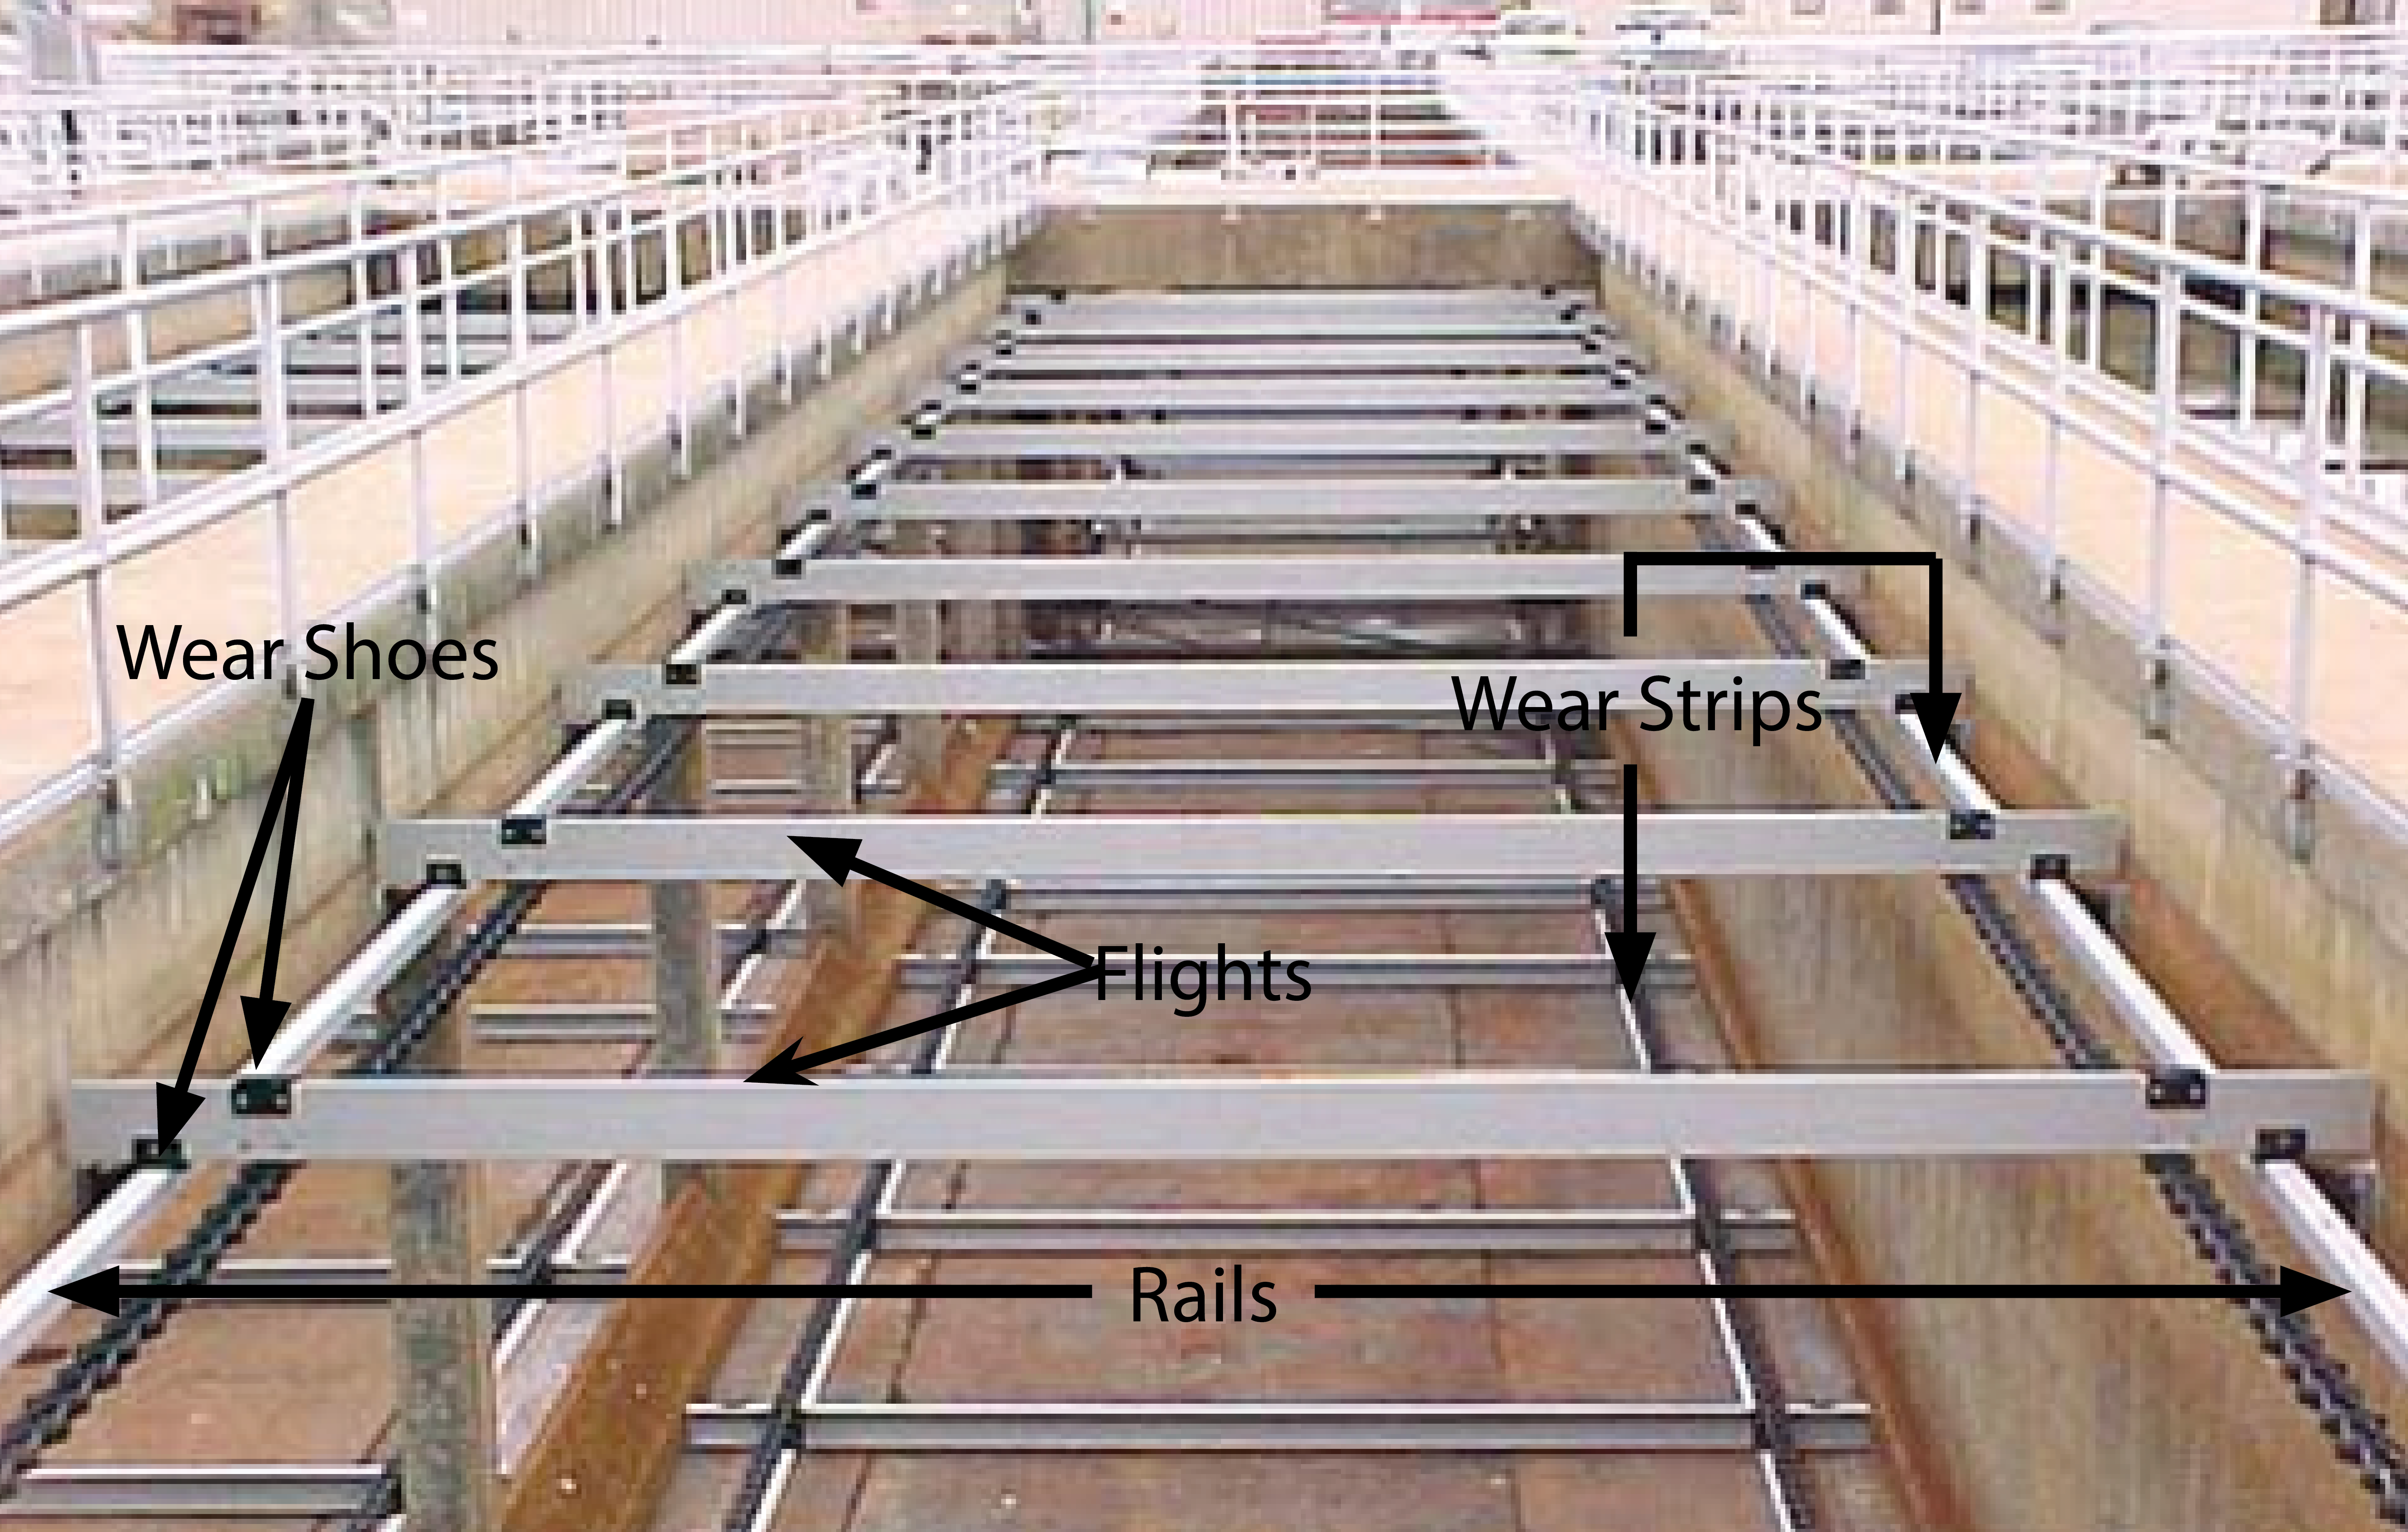
\includegraphics[scale=0.07]												{RectangularClarifierComponents}\\
					Rectangular clarifier flights\\
				\end{center}						  
\end{itemize}
\subsection{Outlet Zone}\index{Outlet Zone}
			\begin{itemize}
				\item  This is the part of the clarifier where the 						settled water leaves to go to the secondary treatment 					processes.
				\item A channel called the effluent launder collects 					the effluent flow and directs it to the primary 						effluent piping. 
				\item Weirs are installed along the edge of the effluent launder channel to skim the water evenly off the surface of the tank. The most common type of effluent weir is a V-notch (or saw-tooth) weir.   A V-	notch weir is a plate that has notches, about 2-3 						inches deep, cut in it every 6-8 inches. If the weir is clean and level, it will remove water evenly all 					the way around the edge of the tank. This minimizes 					the upward velocities near the effluent launder and 					improves removal efficiencies. If the weir plate is not level or part of the weir becomes clogged with 				slime or debris, short-circuiting will result because 					more water will pass over the low side or the clean notches of the weir. Short-circuiting will cause poor 					settling and uneven sludge blanket buildup.
				\item In rectangular tanks the water leaves at the end 	opposite the influent.
												  
				\item In circular  tanks the water leaves at the edge of the tank.
				\item Also, in the circular clarifiers, an effluent baffle, just upstream of the weir, 					is installed to prevent floating solids from going 						over the weir.
\clearpage
				\begin{center}
					\includegraphics[scale=0.04]												{CircularClarifierComponents1}\\
					Circular clarifier skimmer arm, effluent baffle and v-notch weir\\
				\end{center}
				
			\vspace{0.8cm}
					\begin{center}
					\includegraphics[scale=0.07]												{RectangularClarifierWeir}\\
					Rectangular clarifier v-notch weir and launder\\
				\end{center}			
												  
			\end{itemize}

\clearpage
\section{Sludge Pumping}\index{Sludge Pumping}

	\begin{itemize}
		\item The sludge pumping from the clarifier must be adequate 			to prevent sludge from going septic. Septic sludges are much 			more difficult to thicken or de-water and cause odor issues. 
		\item Primary sludge normally averages 4-6\% solids. 
		Generally positive displacement pumps are used for primary 				sludge
		\item The pumping cycles must be designed to provide the 				thickest sludge possible.
		\item Excessive pumping or pumping without building solids to 			build up leads to pumping thinner (more water) sludge.
	\end{itemize}
\section{Design Parameters}\index{Design Parameters}
	\begin{itemize}
	\setlength\itemsep{1em}
		\item \textbf{Clarifier depth} – 8 to 12 feet
		\item \textbf{Hydraulic or surface loading}
			\begin{itemize}
			\item This rate is important to ensure good settleable 					solids removal efficiency
			\item It is expressed in terms of gallons per day per 					square foot (gpd/sq ft) of tank surface area
			\item Typical surface loading rate used for the design of 				primary clarifiers range between 300 to 1,400 gpd/sq ft, 				depending on the nature of the solids and the treatment 				requirements. Lower loading rates are frequently used in 				small plants in cold climates. In warm regions, low rates 				may cause excessive detention which could lead to 						septicity.
			\end{itemize}
	\end{itemize}
	
\section{Advance primary treatment (APT)}\index{Advance primary treatment (APT)}
Synonyms:  Advance primary treatment (APT), Chemically enhanced primary treatment (CEPT), Physical-chemical treatment (Phys-chem)
\subsection{Background}\index{Background}     
      
        \begin{itemize}
			\item Suspended solids present in wastewater are typically coated with bacterial slime and biological metabolic products which are negatively charged.  A significant portion of the suspended solids in wastewater do not settle easily due to gravity as:
				\begin{enumerate}
					\item the biological mass and the associated byproduct gases produced makes these particles buoyant, 
					\item the negative electrostatic charges on these particles cause these particles to be in constant state of motion due to electrostatic repulsion
				\end{enumerate}
			\item Advance primary treatment (APT) also known as Chemically enhanced primary treatment (CEPT) or Physical-chemical treatment (Phys-chem), involves chemical addition to the primary influent flow to enhance primary treatment TSS and BOD removal efficiencies
			\item a normal primary treatment process typically removes 40 to 60\% TSS and 25 to 40\% BOD.  TSS and BOD removal efficiencies of over 80\% and 60\% respectively, may be achieved by the use of APT.
			\item additional cost incurred for the chemical addition is in most cases is offsetted by the benefits which include:
				\begin{enumerate}
					\item by removing more BOD in the primary treatment cost associated with secondary treatment is reduced
					\item primary BOD is more easy to digest than the secondary biomass thus the digester gas production is increased and digested solids production is lowered thus saving biosolids hauling cost
					\item residual ferric chloride in the primary sludge provides H$_2$S and struvite control in the solids treatment processes  
				\end{enumerate}
		\end{itemize}
\vspace{0.4 cm}

\subsection{Process/mechanism}\index{Process/mechanism}    

APT is a two step chemical process:

\textbf{Coagulation}
				                \begin{itemize}
									\item Coagulation is the process by which the negative charge on these particles is reduced lowering the repulsion forces, by the use of a chemical such as ferric chloride and alum.\\
									\item The concentration of the coagulant required is dependent on the strength of the wastewater and the conveyance time of the wastewater.
									\item Typically the coagulant is added immediately after the grit chambers so the conveyance from the grit chambers to the primary clarifier provides adequate contact time and mixing.\\
									\item Parameters to ensure optimal coagulation are:
										\begin{itemize}
											\item Appropriate coagulation concentration
											\item Adequate mixing energy, and
											\item Adequate contact time
										\end{itemize}
									\item Overdosing the coagulant will adversely effect the settleability.
									\item Typical ferric chloride dosage for coagulation range from 12 to 22 mg/l.
								\end{itemize}
\textbf{Flocculation}
			                	\begin{itemize}
									\item Flocculation uses an anionic polymer - polymer which has negatively charged groups, to bridge the coagulated particles to a size which will settle in the primary clarifier.  
									\item The flocculated particles are prone to shearing thus the polymer is gently folded in with the coagulated wastewater just prior to entry into the primary clarifier
								\end{itemize}
					

\vspace{0.6cm}
\hspace{6.8 cm} \textbf{CEPT Schematic}\\
\vspace{0.6cm}
\hspace{1.5 cm}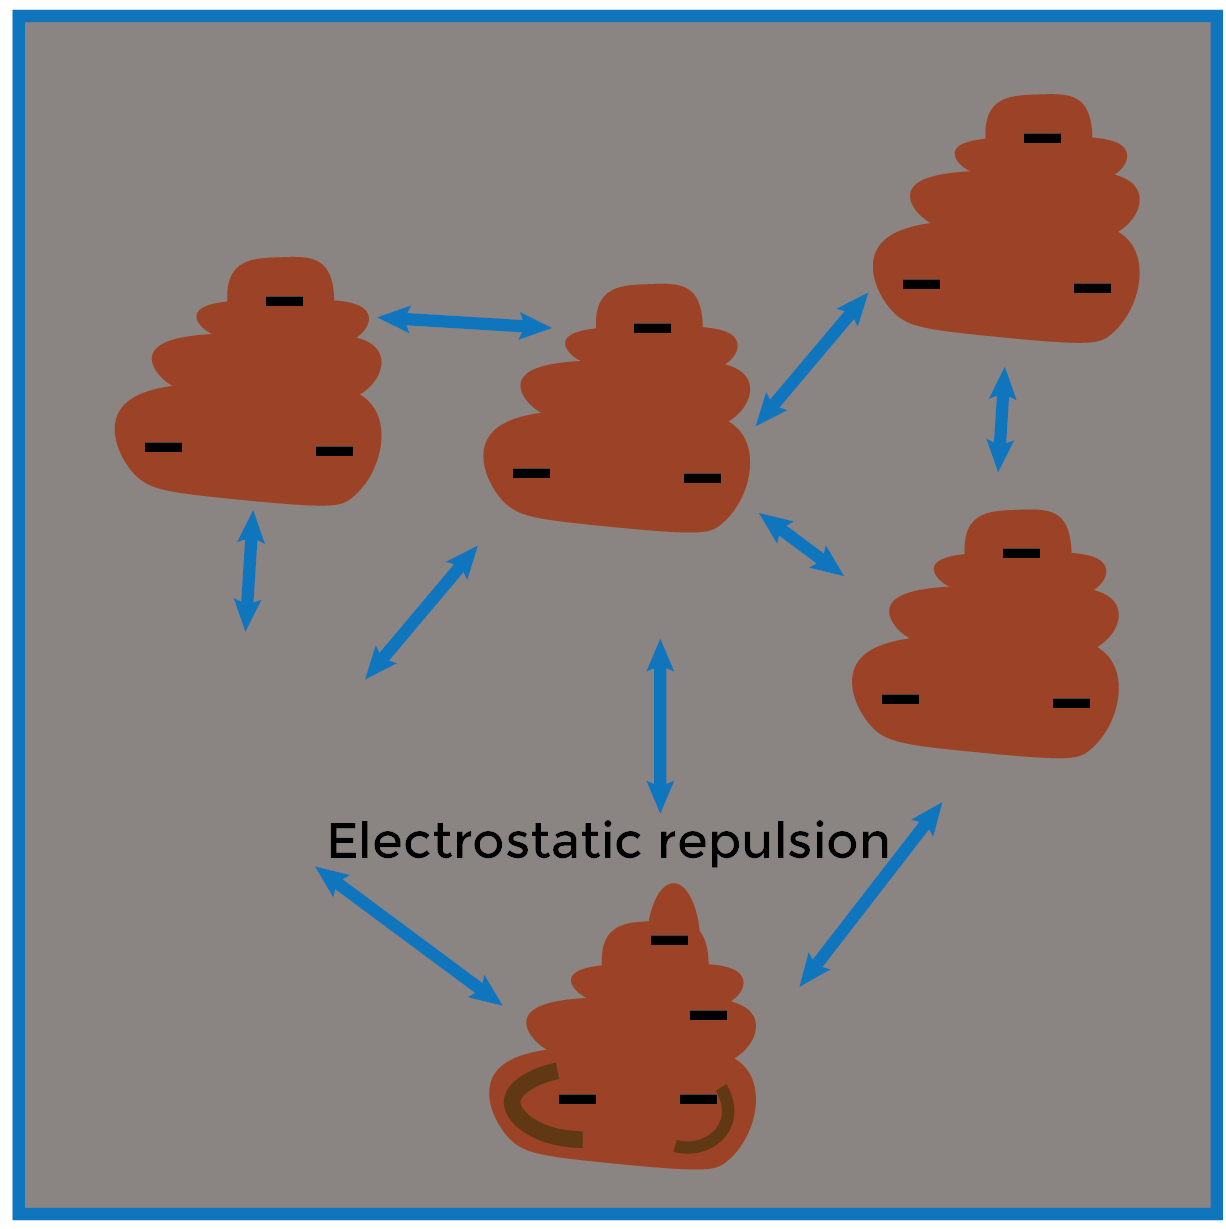
\includegraphics[scale=.13]{CEPTInitial} \hspace{0.7 cm}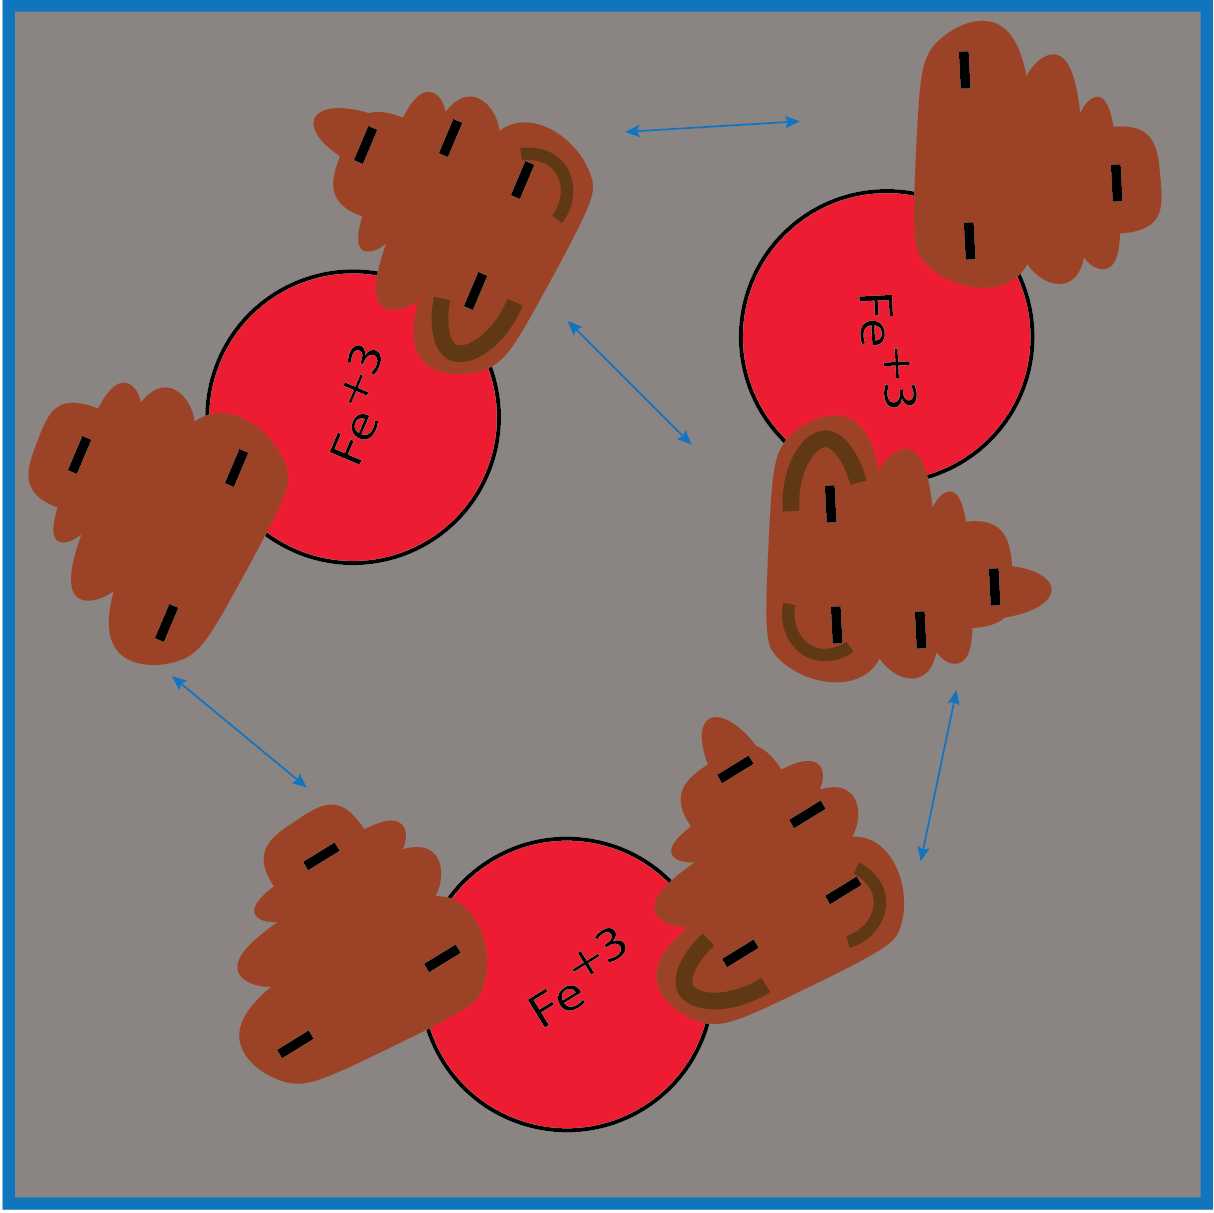
\includegraphics[scale=.13]{CEPTCoagulation}\hspace{0.7 cm}
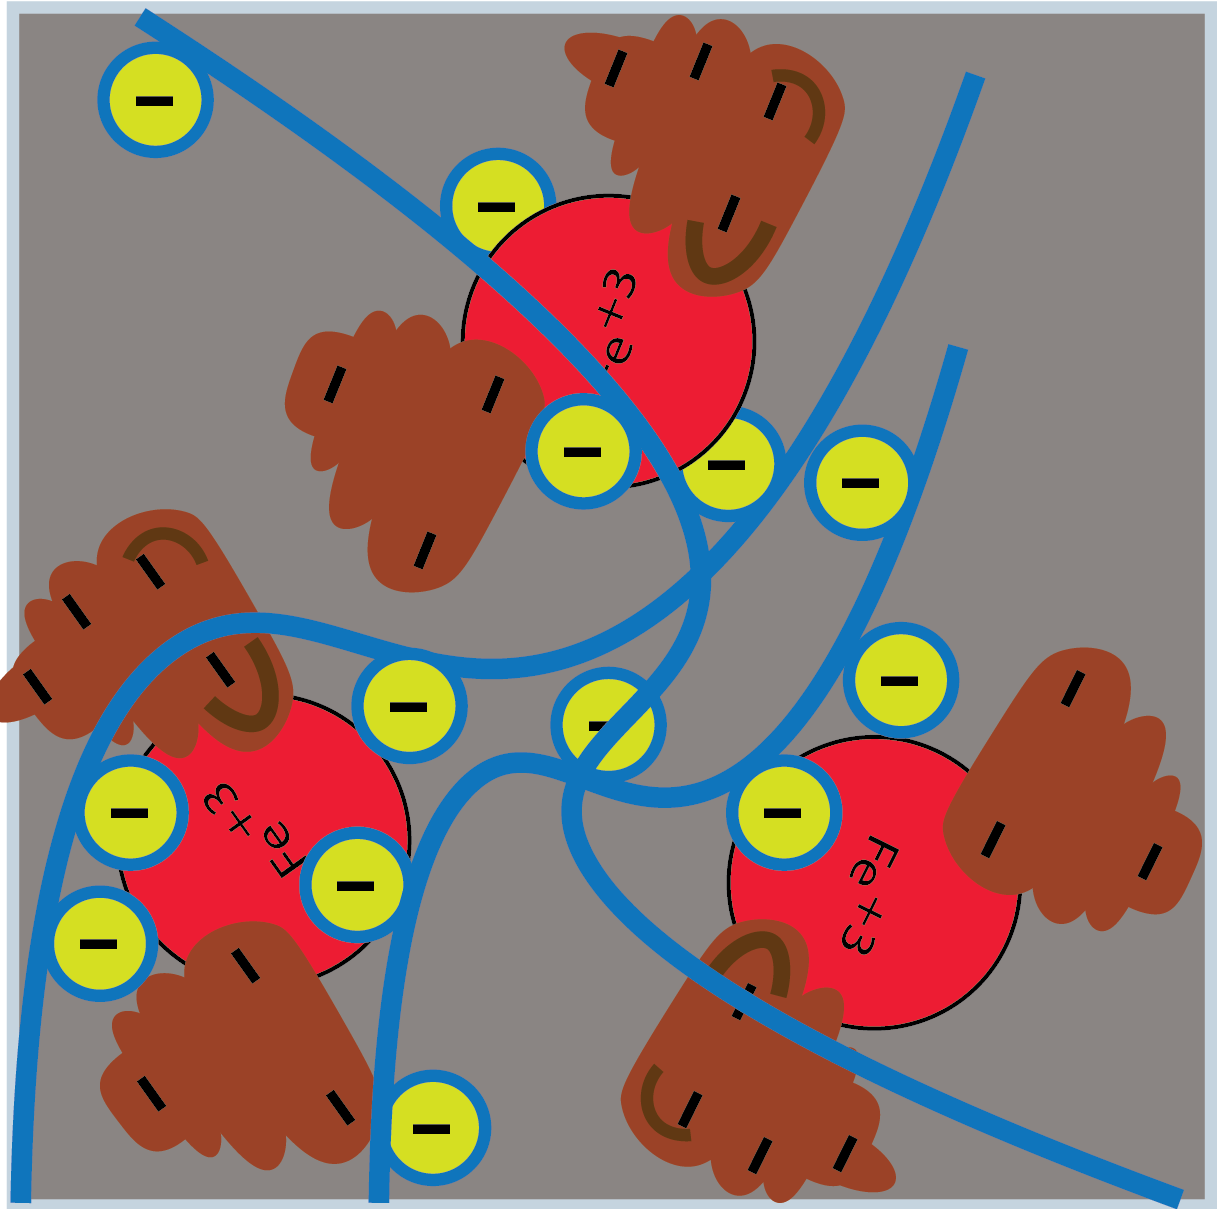
\includegraphics[scale=.13]{CEPTFlocculation}\\
\hspace{0.8 cm} \textbf{Untreated Primary Inluent}\hspace{1.6 cm}\textbf{Coagulation}\hspace{2.8 cm}\textbf{Flocculation}\\	
	
	
	
	
	
\section{Math Problems}\index{Math Problems}

Types of Math Problems Related to Primary Sedimentation 

%\item Finding the clarifier hydraulic or surface loading rate
%\item Finding the clarifier detention time
%\item Finding the clarifier weir overflow rate
%\item Finding the clarifier removal efficiency
%\item Solids removal calculations
%\end{enumerate}
%\begin{enumerate}

\subsection{Hydraulic or Surface Loading Rate}\index{Hydraulic or Surface Loading Rate}

The hydraulic or surface loading rate measures how rapidly wastewater moves through the primary clarifier.  It is measured in terms of the number of gallons flowing each day through one square foot surface area of the clarifier. 
$$Clarifier \enspace hydraulic \enspace loading \enspace 	\Big(\dfrac{gpd}{ft^2}\Big) =\dfrac{Clarifier \enspace influent 	\enspace flow (gpd)}{Clarifier \enspace surface \enspace area 	(ft^2)}$$ 
		Rectangular clarifier surface area  = width * length\\
		Circular clarifier surface area  = 0.785 * Diameter$^2 $\\
\subsection{Detention Time}\index{Detention Time}

Detention time is the length of time that wastewater stays in the settling tank is called the detention time.  It is also the time it takes for a unit volume of wastewater to pass entirely through a primary clarifier\\
$$Clarifier \enspace detention \enspace time \enspace (hr) = 	\dfrac{ Clarifier \enspace volume (cu.ft \enspace or \enspace gal)}{Influent \enspace flow \enspace (cu.ft \enspace or \enspace gal)/hr)}$$
Rectangular clarifier volume = width * length * depth of water\\
Circular clarifier volume = 0.785 * Diameter$^2$ * depth of water\\
Typically volume is calculated in cu. ft and influent flow is given in gallons.  Use 7.48 gal/ft$^3$ conversion factor to convert volume in cu. ft to gallons.\\

\subsection{Weir Overflow Rate}\index{Weir Overflow Rate}
The weirs at the end of the primary clarifier allow for the even distribution of the the outlet flow across the entire length of the weir.  An adequate length of weir is needed to ensure smooth and even flow of wastewater over the weirs.  Weir overflow rate measures the number of gallons of wastewater per day flowing over one foot of weir. 

		$$Weir \enspace over \enspace flow \enspace rate \Big(\dfrac{gpd}{ft}\Big) =\Big(\dfrac{Clarifier \enspace influent \enspace  flow (gpd)}{Total \enspace effluent 					\enspace weir \enspace length \enspace (ft)}\Big)$$
		Circular clarifier weir length = 3.14 * Diameter\\

\hl{Example problem for (a), (b) and (c) above:}\\
		\vspace{0.2cm}
A circular clarifier receives a flow of 11 MGD.  If the clarifier is 90 ft. in diameter and is 12 ft. deep, what is: a) the hydraulic/surface loading rate, b) clarifier detention time in hours, and c) weir overflow rate?\\
		\vspace{0.2cm}
a) Hydraulic/surface loading rate:\\
$Clarifier \enspace hydraulic \enspace loading \enspace 	\Big(\dfrac{gpd}{ft^2}\Big) ==\dfrac{\dfrac{11\cancel{MG}}{{day}}*\dfrac{10^6gal}{\cancel{MG}}}{0.785*90^2 ft^2}=\boxed{1,730gpd/ft^2}$\\
		\vspace{0.5cm}
b) Clarifier detention time:\\
$Clarifier \enspace detention \enspace time \enspace (hr) = 	\dfrac{ Clarifier \enspace volume (cu.ft \enspace or \enspace gal)}{Influent \enspace flow \enspace (cu.ft \enspace or \enspace gal)/hr)}$\\
		\vspace{0.2cm}
$Clarifier \enspace detention \enspace time \enspace (hr) = 	\dfrac{(0.785*90^2*12)\cancel{ft^3}}{\dfrac{11\cancel{MG}}{\cancel{day}}*\dfrac{10^6\cancel{gal}}{\cancel{MG}}*\dfrac{\cancel{ft^3}}{7.48\cancel{gal}}*\dfrac{\cancel{day}}{24hrs}}=\boxed{1.2hrs}$\\
		\vspace{0.5cm}
c) Weir overflow rate:\\
		\vspace{0.2cm} 
$Weir \enspace overflow \enspace rate \Big(\dfrac{gpd}{ft}\Big) =\dfrac{\dfrac{11\cancel{MG}}{{day}}*\dfrac{10^6gal}{\cancel{MG}}}{3.14*90 ft}=\boxed{38,924gpd/ft}$\\

\subsection{Removal Efficiency}\index{Removal Efficiency}		
Primary sedimentation removes suspended wastewater solids which includes BOD.  The efficiency of the primary is established as the percentage of the amount of parameter removed.  The parameter may quantified as mass (lbs) or as concentration (mg/l).

$$Removal \enspace efficiency (\%) = \dfrac{Parameter  \enspace In - Parameter  \enspace Out}{Parameter \enspace In} * 100$$

For TSS removal:\\
$$TSS \enspace Removal \enspace efficiency (\%) = \dfrac{TSS  _{In} \enspace(mg/l)  - TSS_{Out} \enspace(mg/l)  }{TSS _{In} \enspace(mg/l)  } * 100$$

For BOD removal:\\
$$BOD \enspace Removal \enspace efficiency (\%) = \dfrac{BOD_{In} \enspace(mg/l)  - BOD_{Out} \enspace(mg/l)  }{BOD _{In} \enspace(mg/l)  } * 100$$
\subsection{Solids Removal}\index{Solids Removal}	

\hl{\textbf{Type 1 Problems:}  These involve calculating lbs of solids removed given any two of the following TSS parameters - inlet concentration, outlet concentration and removal efficiency.}\\
a. If the inlet and outlet concentrations are given, calculate the mg/l of TSS removed using: 
$$TSS_{removed} = TSS_{in}(mg/l) - TSS_{out} (mg/l) $$
Then knowing the flow, use the lbs formula to calculate the lbs solids removed.

b. If either inlet or outlet concentration is given along with the clarifier removal efficiency, using the removal efficiency calculate the unknown outlet concentration (if only the inlet is given) or the inlet concentration (if only the outlet is given)\\
i) If inlet and removal efficiency is given, calculate the outlet by subtracting the product of inlet and removal efficiency from the inlet.
$$TSS_{out}=TSS_{in} - (TSS_{in}*\%Removal)$$
Example if the removal efficiency is 60\% and the inlet concentration is 300mg/l: $$TSS_{out}=300 - 300*0.6=120mg/l$$
ii) If outlet and removal efficiency is given, calculate the inlet concentration by dividing the outlet by (1-removal efficiency).\\
$$TSS_{in}=\dfrac{TSS_{out}}{1-\%Removal}$$
Example if the removal efficiency is 60\% and the outlet concentration is 120mg/l: $$TSS_{in}=\dfrac{120}{1-0.6}=300mg/l$$ 

Note:  You may derive the above formulas by algebraically manipulating: $\%Removal=\dfrac{TSS_{in} -TSS_{out}}{TSS_{in}}$\\
\hl{Example Problem:}\\
How many lbs of solids are removed daily by a primary clarifier treating a 6 MGD flow if the average influent TSS concentration is 300 mg/l and the clarifier TSS removal efficiency is 67\%.\\
$TSS_{out}=(300mg/l - 300*0.67)=99mg/l$\\
$lbs \enspace solids \enspace  removed = (300-99)mg/l*8.34*6MGD=\boxed{10,058 \enspace lbs \enspace solids \enspace removed \enspace per \enspace day}$\\
\vspace{0.5cm}
\hl{\textbf{Type 2 Problems:}  These involve calculating the amount of sludge pumping given the solids removed.  The solids removed from the primary clarifier is sludge with a typical solids concentration of about 3\% to 5\%.}\\
Given the amount of total solids removed and given the sludge concentration, the volume of sludge pumping can be calculated as follows:  $$\dfrac{ft^3\enspace sludge\enspace pumped}{ day}= \dfrac{lbs \enspace solids \enspace (removed)}{day} * \dfrac{1 \enspace lb \enspace sludge}{(\%)\enspace lbs \enspace solids}*\dfrac{gal \enspace sludge}{8.34lb \enspace sludge}*\dfrac{ft^3 \enspace sludge}{7.48 \enspace gal} $$
So for the solids removed in the above example, if the primary sludge has 5\% solids, the required sludge pumping can be calculated as:
$$\dfrac{ft^3\enspace sludge}{day}= \dfrac{10,058 \enspace \cancel{lbs \enspace solids}}{day} * \dfrac{1 \enspace \cancel{lb \enspace sludge}}{0.05\enspace \cancel{lbs \enspace solids}}*\dfrac{\cancel{gal \enspace sludge}}{8.34\cancel{lb \enspace sludge}}*\dfrac{ft^3 \enspace sludge}{7.48 \enspace \cancel{gal}}=\boxed{3,224\dfrac{ft^3 \enspace sludge}{day}} $$
